\documentclass[10pt,a4paper]{article}

% ===== Kodowanie i język =====
\usepackage[T1]{fontenc}
\usepackage[utf8]{inputenc}
\usepackage[polish]{babel}
\usepackage{lmodern}

% ===== Układ strony =====
\usepackage[a4paper,margin=1.5cm]{geometry}

% ===== Matematyka =====
\usepackage{amsmath, amssymb, amsfonts, amsthm, mathtools}

% ===== Grafika i rysunki =====
\usepackage{graphicx}
\usepackage{float}
\usepackage{xcolor}
\usepackage{tikz}
\usetikzlibrary{positioning}

% ===== Algorytmy =====
\usepackage{algorithm}
\usepackage{algpseudocode}

% ===== Listy =====
\usepackage{enumitem}

% ===== Linki =====
\usepackage{hyperref}


% ===== Cytowania i bibliografia =====
\usepackage{csquotes}
\usepackage[backend=biber,style=numeric]{biblatex}
\addbibresource{bibliography.bib}

% ===== Skróty matematyczne =====
\newcommand{\R}{\mathbb{R}}
\newcommand{\Z}{\mathbb{Z}}
\newcommand{\N}{\mathbb{N}}
\newcommand{\Q}{\mathbb{Q}}
\newcommand{\C}{\mathbb{C}}
\newcommand{\D}{\mathcal{D}}
\newcommand{\F}{\mathbb{F}}
\newcommand{\plate}[1]{\raisebox{-0.35\height}{\includegraphics[height=1.8em]{#1}}}
\newcommand{\EmptyBar}{\plate{images/pusta.jpg}}
\newcommand{\SetA}{\{\plate{images/0,25.png},\plate{images/0,5.png},\plate{images/1,25.png}\}}
\newcommand{\SetB}{\{\plate{images/2,5.png},\plate{images/5.png}\}}
\newcommand{\SetC}{\{\plate{images/10.png},\plate{images/15.png},\plate{images/20.png},\plate{images/25.png}\}}
\newcommand{\SetAB}{\{\plate{images/0,25.png},\plate{images/0,5.png},\plate{images/1,25.png},\plate{images/2,5.png},\plate{images/5.png}\}}
\newcommand{\SetAC}{\{\plate{images/0,25.png},\plate{images/0,5.png},\plate{images/1,25.png},\plate{images/10.png},\plate{images/15.png},\plate{images/20.png},\plate{images/25.png}\}}
\newcommand{\SetBC}{\{\plate{images/2,5.png},\plate{images/5.png},\plate{images/10.png},\plate{images/15.png},\plate{images/20.png},\plate{images/25.png}\}}
\newcommand{\SetX}{\{\plate{images/0,25.png},\plate{images/0,5.png},\plate{images/1,25.png},\plate{images/2,5.png},\plate{images/5.png},\plate{images/10.png},\plate{images/15.png},\plate{images/20.png},\plate{images/25.png}\}}

% ===== Środowiska twierdzeń =====
\theoremstyle{plain}
\newtheorem{tw}{Twierdzenie}[section]
\newtheorem{lem}[tw]{Lemat}
\newtheorem{wn}[tw]{Wniosek}

\theoremstyle{definition}
\newtheorem{df}[tw]{Definicja}
\newtheorem{uw}[tw]{Uwaga}
\newtheorem{prz}[tw]{Przykład}

% ===== Ustawienia linków =====
\hypersetup{
    colorlinks=true,
    linkcolor=blue,
    citecolor=blue,
    urlcolor=blue
}

\title{Topologia Talerzy Eleiko}
\author{Paweł Drzyzga}
\date{31 marca 2026}

\begin{document}

\maketitle
% \tableofcontents

\section{Aksjomaty topologii}

\begin{df}[Topologia]
Niech $X$ będzie niepustym zbiorem. Rodzinę podzbiorów $\mathcal{T} \subseteq \mathcal{P}(X)$
nazywamy \emph{topologią} na $X$, jeśli spełnione są trzy aksjomaty:
\begin{enumerate}[label=(T\arabic*)]
    \item $\emptyset \in \mathcal{T}$ oraz $X \in \mathcal{T}$,
    \item dla dowolnej rodziny $\{U_i\}_{i \in I} \subseteq \mathcal{T}$ mamy
    $\bigcup_{i \in I} U_i \in \mathcal{T}$,
    \item dla dowolnych $U_1,\dots,U_n \in \mathcal{T}$ mamy
    $\bigcap_{k=1}^{n} U_k \in \mathcal{T}$.
\end{enumerate}
Elementy rodziny $\mathcal{T}$ nazywamy zbiorami otwartymi.
\end{df}

\begin{uw}
W metaforze siłowni aksjomat (T1) mówi, że dopuszczamy zarówno sytuację ``pusta sztanga''
($\emptyset$), jak i pełny zestaw talerzy ($X$). Aksjomat (T2) pozwala łączyć dowolnie wiele
dozwolonych konfiguracji, a (T3) zapewnia, że część wspólna skończonej liczby konfiguracji
nadal pozostaje dozwolona.
\end{uw}

\begin{prz}[Dlaczego przekroje muszą być skończone?]
W praktyce treningowej można narzucić kilka jednoczesnych warunków, na przykład:
``bierzemy tylko talerze do rozgrzewki'' oraz ``bierzemy tylko talerze z prawej strony stojaka''.
Wspólny fragment takich warunków ma sens i powinien pozostać dozwoloną konfiguracją.
To intuicyjnie tłumaczy aksjomat (T3).
\end{prz}

\section{Historyjka: stojak, talerze i porządek}

Wyobraźmy sobie stojak na talerze na siłowni. Każdy talerz to jeden punkt naszej przestrzeni,
a cały zestaw talerzy to przestrzeń $X$. Chcemy opisać, które grupy talerzy uznajemy za
``naturalnie dostępne'' bez rozbijania układu. W języku topologii takie grupy to zbiory otwarte.

Intuicja jest taka: jeśli raz uznamy pewne konfiguracje talerzy za sensowne, to możemy je
bezpiecznie łączyć i porównywać bez utraty porządku. Nawet przypadek, gdy na sztandze nie ma
żadnego talerza, jest ważny w opisie: narracyjnie mówimy wtedy o pustej sztandze, a formalnie
to po prostu zbiór pusty $\emptyset$.

\begin{figure}[H]
    \centering
    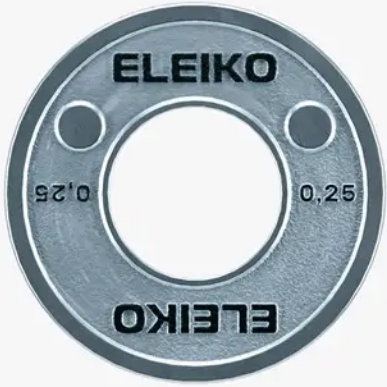
\includegraphics[width=0.18\textwidth]{images/0,25.png}\hfill
    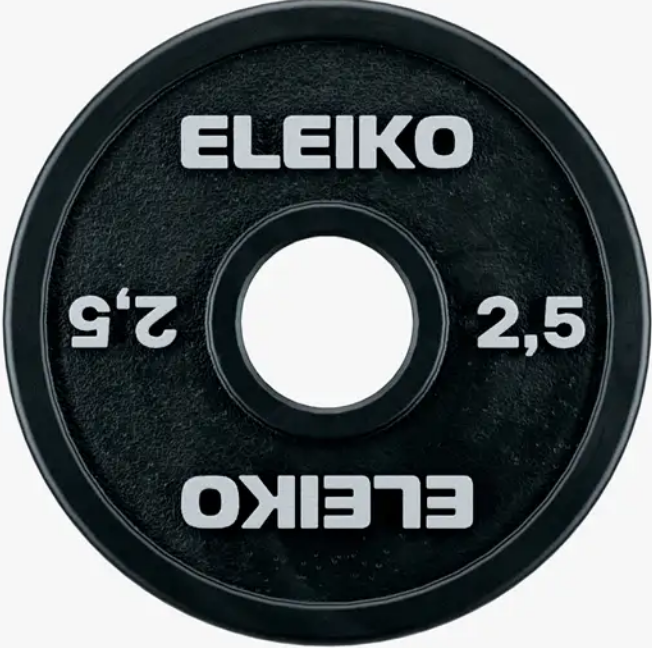
\includegraphics[width=0.18\textwidth]{images/2,5.png}\hfill
    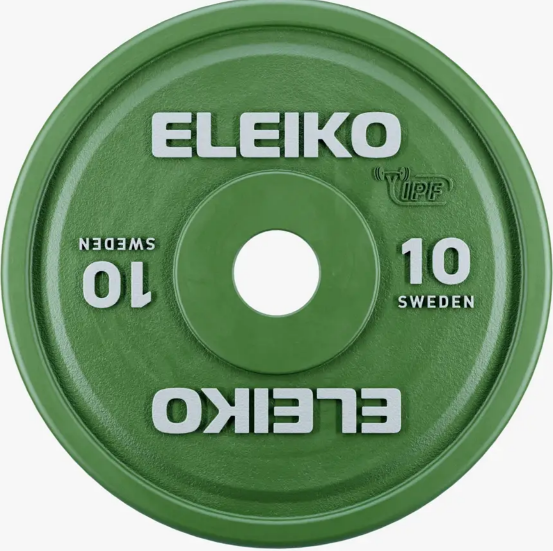
\includegraphics[width=0.18\textwidth]{images/10.png}\hfill
    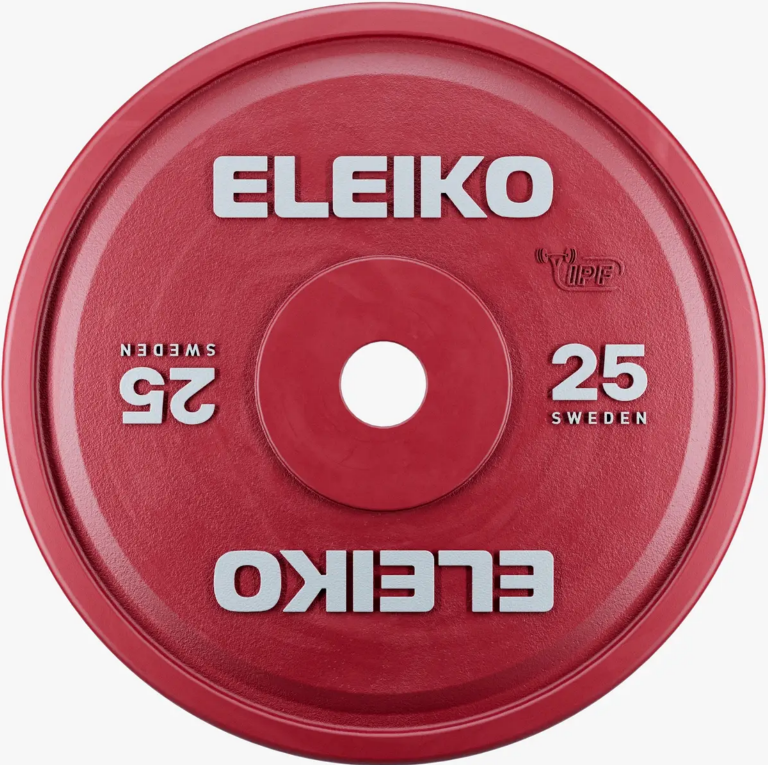
\includegraphics[width=0.18\textwidth]{images/25.png}
    \caption{Przykładowe ``punkty'' przestrzeni: talerze o różnych masach.}
\end{figure}

W tym projekcie traktujemy topologię jako zasady, które mówią, jak budować sensowne rodziny
konfiguracji talerzy: od bardzo lekkich, przez mieszane, aż po ciężkie zestawy.

\section{Zbiór talerzy}

W tej sekcji precyzyjnie definiujemy nasz model: określamy zbiór $X$ wszystkich talerzy
oraz rodzinę $\mathcal{T}$ zbiorów otwartych stanowiących topologię.

\begin{prz}[Nasz zbiór $X$ i rodzina $\mathcal{T}$]
Niech
\[
X = \{\plate{images/0,25.png},\plate{images/0,5.png},\plate{images/1,25.png},\plate{images/2,5.png},
\plate{images/5.png},\plate{images/10.png},\plate{images/15.png},\plate{images/20.png},\plate{images/25.png}\}
\]
oznacza zestaw obiektów treningowych zapisanych bezpośrednio przez grafiki.
Obrazek \plate{images/pusta.jpg} interpretujemy wyłącznie jako ikonę zbioru pustego $\emptyset$,
czyli pustą sztangę, a nie jako element zbioru $X$.

Rozważmy rodzinę
\[
\begin{aligned}
\mathcal{T} = \Big\{&
\plate{images/pusta.jpg},\\
&\{\plate{images/0,25.png},\plate{images/0,5.png},\plate{images/1,25.png}\},\\
&\{\plate{images/2,5.png},\plate{images/5.png}\},\\
&\{\plate{images/10.png},\plate{images/15.png},\plate{images/20.png},\plate{images/25.png}\},\\
&\{\plate{images/0,25.png},\plate{images/0,5.png},\plate{images/1,25.png},\plate{images/2,5.png},\plate{images/5.png}\},\\
&\{\plate{images/0,25.png},\plate{images/0,5.png},\plate{images/1,25.png},\plate{images/10.png},\plate{images/15.png},\plate{images/20.png},\plate{images/25.png}\},\\
&\{\plate{images/2,5.png},\plate{images/5.png},\plate{images/10.png},\plate{images/15.png},\plate{images/20.png},\plate{images/25.png}\},\\
&\{\plate{images/0,25.png},\plate{images/0,5.png},\plate{images/1,25.png},\plate{images/2,5.png},\plate{images/5.png},\plate{images/10.png},\plate{images/15.png},\plate{images/20.png},\plate{images/25.png}\}
\Big\}
\end{aligned}
\]
czyli mamy trzy podstawowe bloki otwarte: \emph{technika}, \emph{stabilizacja} i \emph{moc},
oraz ich kombinacje przez sumy.
\end{prz}

\section{Sprawdzenie, czy zadany model T jest topologią}

\[
\begin{aligned}
\mathcal{T} = \Big\{&
\plate{images/pusta.jpg},\\
&\{\plate{images/0,25.png},\plate{images/0,5.png},\plate{images/1,25.png}\},\\
&\{\plate{images/2,5.png},\plate{images/5.png}\},\\
&\{\plate{images/10.png},\plate{images/15.png},\plate{images/20.png},\plate{images/25.png}\},\\
&\{\plate{images/0,25.png},\plate{images/0,5.png},\plate{images/1,25.png},\plate{images/2,5.png},\plate{images/5.png}\},\\
&\{\plate{images/0,25.png},\plate{images/0,5.png},\plate{images/1,25.png},\plate{images/10.png},\plate{images/15.png},\plate{images/20.png},\plate{images/25.png}\},\\
&\{\plate{images/2,5.png},\plate{images/5.png},\plate{images/10.png},\plate{images/15.png},\plate{images/20.png},\plate{images/25.png}\},\\
&\{\plate{images/0,25.png},\plate{images/0,5.png},\plate{images/1,25.png},\plate{images/2,5.png},\plate{images/5.png},\plate{images/10.png},\plate{images/15.png},\plate{images/20.png},\plate{images/25.png}\}
\Big\}
\end{aligned}
\]

\begin{figure}[H]
    \centering
    \renewcommand{\arraystretch}{1.35}
    \begin{tabular}{l}
    $\tau_1=\EmptyBar$ \\
    $\tau_2=\SetA$ \\
    $\tau_3=\SetB$ \\
    $\tau_4=\SetC$ \\
    $\tau_5=\SetAB$ \\
    $\tau_6=\SetAC$ \\
    $\tau_7=\SetBC$ \\
    $\tau_8=\SetX$
    \end{tabular}
    \caption{Całe $\mathcal{T}$: wszystkie 8 zbiorów otwartych zapisane obrazkami.}
\end{figure}

\subsection*{I.}
\[
\EmptyBar\in\mathcal{T}\ \checkmark
\qquad\qquad
\SetX\in\mathcal{T}\ \checkmark
\]

\subsection*{II.}
\[
\SetA\cap\SetB=\EmptyBar\ \checkmark
\]
\[
\SetA\cap\SetC=\EmptyBar\ \checkmark
\]
\[
\SetB\cap\SetC=\EmptyBar\ \checkmark
\]
\[
\SetAB\cap\SetAC=\SetA\ \checkmark
\]
\[
\SetAC\cap\SetBC=\SetC\ \checkmark
\]

\begin{figure}[H]
    \centering
    \begin{tikzpicture}[node distance=1.5cm and 1.8cm, every node/.style={draw, rounded corners, align=center, inner sep=3pt, font=\small}]
        \node (X) {$\SetX$};
        \node (AB) [below left=of X] {$\SetAB$};
        \node (AC) [below=of X] {$\SetAC$};
        \node (BC) [below right=of X] {$\SetBC$};

        \node (A) [below left=of AC] {$\SetA$};
        \node (B) [below=of AC] {$\SetB$};
        \node (C) [below right=of AC] {$\SetC$};

        \node (E) [below=of B] {$\EmptyBar$};

        \draw (AB)--(X);
        \draw (AC)--(X);
        \draw (BC)--(X);

        \draw (A)--(AB);
        \draw (B)--(AB);
        \draw (A)--(AC);
        \draw (C)--(AC);
        \draw (B)--(BC);
        \draw (C)--(BC);

        \draw (E)--(A);
        \draw (E)--(B);
        \draw (E)--(C);
    \end{tikzpicture}
    \caption{Kratowy obraz całego $\mathcal{T}$.}
\end{figure}

\subsection*{III.}
\[
\SetA\cup\SetB=\SetAB\ \checkmark
\]
\[
\SetA\cup\SetC=\SetAC\ \checkmark
\]
\[
\SetB\cup\SetC=\SetBC\ \checkmark
\]
\[
\SetA\cup\SetB\cup\SetC=\SetX\ \checkmark
\]

\[
\boxed{\mathcal{T}\ \text{jest topologią na}\ X}\quad\checkmark
\]

\section{Talerzowa funkcja ciagla}

\subsection*{Definicja ciaglosci funkcji}
\[
F:(X,\mathcal{T})\to(X,\mathcal{T})
\]
\[
\forall U\in\mathcal{T}\quad F^{-1}(U)\in\mathcal{T}
\]

\subsection*{Model graficzny}
\[
\text{Dynamika dzieje sie na tym samym zbiorze }X\text{, wiec mozemy iterowac }F^n(x).
\]

\[
F(x)=
\begin{cases}
\plate{images/0,5.png}, & x=\plate{images/0,25.png},\\
\plate{images/1,25.png}, & x=\plate{images/0,5.png},\\
\plate{images/0,25.png}, & x=\plate{images/1,25.png},\\
\plate{images/5.png}, & x=\plate{images/2,5.png},\\
\plate{images/2,5.png}, & x=\plate{images/5.png},\\
\plate{images/15.png}, & x=\plate{images/10.png},\\
\plate{images/20.png}, & x=\plate{images/15.png},\\
\plate{images/25.png}, & x=\plate{images/20.png},\\
\plate{images/10.png}, & x=\plate{images/25.png}.
\end{cases}
\]

\begin{figure}[H]
    \centering
    \begin{tikzpicture}[node distance=1.4cm, every node/.style={draw, rounded corners, inner sep=5pt}]
        % Blok A: cykl dlugosci 3
        \node (a1) at (0, 1.6) {\plate{images/0,25.png}};
        \node (a2) [right=of a1] {\plate{images/0,5.png}};
        \node (a3) [right=of a2] {\plate{images/1,25.png}};
        \draw[->, thick, red!70] (a1) -- (a2);
        \draw[->, thick, red!70] (a2) -- (a3);
        \draw[->, thick, red!70, bend left=30] (a3) to (a1);

        % Blok B: cykl dlugosci 2
        \node (b1) at (0, 0) {\plate{images/2,5.png}};
        \node (b2) [right=of b1] {\plate{images/5.png}};
        \draw[->, thick, blue!70] (b1) -- (b2);
        \draw[->, thick, blue!70, bend left=35] (b2) to (b1);

        % Blok C: cykl dlugosci 4
        \node (c1) at (0, -1.8) {\plate{images/10.png}};
        \node (c2) [right=of c1] {\plate{images/15.png}};
        \node (c3) [right=of c2] {\plate{images/20.png}};
        \node (c4) [right=of c3] {\plate{images/25.png}};
        \draw[->, thick, green!60!black] (c1) -- (c2);
        \draw[->, thick, green!60!black] (c2) -- (c3);
        \draw[->, thick, green!60!black] (c3) -- (c4);
        \draw[->, thick, green!60!black, bend right=25] (c4) to (c1);
    \end{tikzpicture}
    \caption{Graf funkcji $F: (X, \mathcal{T}) \to (X, \mathcal{T})$ zapisanej jako cykle w blokach $A,B,C$.}
\end{figure}

\begin{figure}[H]
    \centering
    \begin{tikzpicture}[scale=0.88]
        % Osie
        \draw[->, thick] (0,0) -- (10.2,0) node[right] {$x\in X$};
        \draw[->, thick] (0,0) -- (0,9.8) node[above] {$F(x)\in X$};

        % Punkty i etykiety na osi X
        \foreach \x/\img in {
            1/{images/0,25.png},
            1.9/{images/0,5.png},
            2.8/{images/1,25.png},
            3.7/{images/2,5.png},
            4.6/{images/5.png},
            5.8/{images/10.png},
            6.8/{images/15.png},
            7.8/{images/20.png},
            8.8/{images/25.png}}
        {
            \draw[thick, fill] (\x,0) circle (1.7pt);
            \node at (\x,-0.45) {\tiny \plate{\img}};
        }

        % Punkty i etykiety na osi Y
        \foreach \y/\img in {
            1/{images/0,25.png},
            2/{images/0,5.png},
            3/{images/1,25.png},
            4/{images/2,5.png},
            5/{images/5.png},
            6/{images/10.png},
            7/{images/15.png},
            8/{images/20.png},
            9/{images/25.png}}
        {
            \draw[thick, fill] (0,\y) circle (1.7pt);
            \node at (-0.75,\y) {\tiny \plate{\img}};
        }

        % Punkty wykresu y = F(x)
        \draw[thick, fill, color=red!70] (1,2) circle (2pt);
        \draw[thick, fill, color=red!70] (1.9,3) circle (2pt);
        \draw[thick, fill, color=red!70] (2.8,1) circle (2pt);

        \draw[thick, fill, color=blue!70] (3.7,5) circle (2pt);
        \draw[thick, fill, color=blue!70] (4.6,4) circle (2pt);

        \draw[thick, fill, color=green!60!black] (5.8,7) circle (2pt);
        \draw[thick, fill, color=green!60!black] (6.8,8) circle (2pt);
        \draw[thick, fill, color=green!60!black] (7.8,9) circle (2pt);
        \draw[thick, fill, color=green!60!black] (8.8,6) circle (2pt);
    \end{tikzpicture}
    \caption{Wykres funkcji $F$ w stylu osiowym: kazdemu talerzowi $x$ odpowiada punkt $(x,F(x))$.}
\end{figure}

\subsection*{Czy F jest ciagla?}
\[
F^{-1}(\EmptyBar)=\EmptyBar\in\mathcal{T}\ \checkmark
\]
\[
F^{-1}(\{\plate{images/0,5.png}\})=\SetA\in\mathcal{T}\ \checkmark
\]
\[
F^{-1}(\{\plate{images/5.png}\})=\SetB\in\mathcal{T}\ \checkmark
\]
\[
F^{-1}(\{\plate{images/20.png}\})=\SetC\in\mathcal{T}\ \checkmark
\]
\[
F^{-1}(\{\plate{images/0,5.png},\plate{images/5.png}\})=\SetAB\in\mathcal{T}\ \checkmark
\]
\[
F^{-1}(\{\plate{images/0,5.png},\plate{images/20.png}\})=\SetAC\in\mathcal{T}\ \checkmark
\]
\[
F^{-1}(\{\plate{images/5.png},\plate{images/20.png}\})=\SetBC\in\mathcal{T}\ \checkmark
\]
\[
F^{-1}(\SetX)=\SetX\in\mathcal{T}\ \checkmark
\]

\[
\boxed{F\ \text{jest ciagla}}\quad\checkmark
\]

\section{Trajektoria}

\subsection*{Uklad Dynamiczny}

Iterujemy funkcję $F$ wielokrotnie, budując trajektorię:

\[
\begin{aligned}
\text{Trj. 1:}\quad &\plate{images/0,25.png} \xrightarrow{F} \plate{images/0,5.png} \xrightarrow{F} \plate{images/1,25.png} \xrightarrow{F} \plate{images/0,25.png} \xrightarrow{F} \cdots\\
\text{Trj. 2:}\quad &\plate{images/2,5.png} \xrightarrow{F} \plate{images/5.png} \xrightarrow{F} \plate{images/2,5.png} \xrightarrow{F} \plate{images/5.png} \xrightarrow{F} \cdots\\
\text{Trj. 3:}\quad &\plate{images/10.png} \xrightarrow{F} \plate{images/15.png} \xrightarrow{F} \plate{images/20.png} \xrightarrow{F} \plate{images/25.png} \xrightarrow{F} \cdots
\end{aligned}
\]

Okres trajektorii 1 wynosi $3$, trajektorii 2 wynosi $2$, a trajektorii 3 wynosi $4$.

\subsection*{Orbity Trajektorii}

Orbity wyznaczane przez trajektorie to następujące zbiory:

\[
\{\plate{images/0,25.png}, \plate{images/0,5.png}, \plate{images/1,25.png}\},
\qquad
\{\plate{images/2,5.png}, \plate{images/5.png}\},
\qquad
\{\plate{images/10.png}, \plate{images/15.png}, \plate{images/20.png}, \plate{images/25.png}\}
\]

\subsection*{Wykres Trajektorii Talerzy}

\begin{figure}[H]
    \centering
    \begin{tikzpicture}[scale=1, node distance=1.2cm, every node/.style={draw, rounded corners, align=center, inner sep=6pt, font=\small}]
        % Trajektoria 1
        \node (t1a) at (0, 2) {\plate{images/0,25.png}};
        \node (t1b) [right=of t1a] {\plate{images/0,5.png}};
        \node (t1c) [right=of t1b] {\plate{images/1,25.png}};
        \draw[->, thick] (t1a) -- (t1b);
        \draw[->, thick] (t1b) -- (t1c);
        \draw[->, thick, bend left=30] (t1c) to (t1a);
        
        % Trajektoria 2
        \node (t2a) at (0, 0.5) {\plate{images/2,5.png}};
        \node (t2b) [right=of t2a] {\plate{images/5.png}};
        \node (t2c) [right=of t2b] {\plate{images/2,5.png}};
        \draw[->, thick] (t2a) -- (t2b);
        \draw[->, thick] (t2b) -- (t2c);
        \draw[->, thick, bend left=30] (t2c) to (t2a);
        
        % Trajektoria 3
        \node (t3a) at (0, -1) {\plate{images/10.png}};
        \node (t3b) [right=of t3a] {\plate{images/15.png}};
        \node (t3c) [right=of t3b] {\plate{images/20.png}};
        \node (t3d) [right=of t3c] {\plate{images/25.png}};
        \draw[->, thick] (t3a) -- (t3b);
        \draw[->, thick] (t3b) -- (t3c);
        \draw[->, thick] (t3c) -- (t3d);
        \draw[->, thick, bend right=22] (t3d) to (t3a);
    \end{tikzpicture}
    \caption{Trajektorie i orbity funkcji $F$ na zbiorze talerzy.}
\end{figure}

\section{Podsumowanie}

W projekcie zbudowaliśmy pełny model topologiczno-dynamiczny dla zbioru talerzy siłowych.
Najpierw określiliśmy przestrzeń $(X,\mathcal{T})$ i zweryfikowaliśmy aksjomaty topologii,
czyli domknięcie na sumy, przekroje skończone oraz obecność $\emptyset$ i $X$.

Następnie zdefiniowaliśmy funkcję
\[
F:(X,\mathcal{T})\to(X,\mathcal{T}),
\]
co pozwoliło jednocześnie badać jej ciągłość (przez preobrazy zbiorów otwartych)
oraz dynamikę iteracji $F^n(x)$. Dzięki temu trajektorie i orbity są merytorycznie
spójne z definicją funkcji: dostajemy cykle o okresach $3$, $2$ i $4$.

Model pokazuje, że abstrakcyjne pojęcia topologii i układów dynamicznych można opisać
w czytelny, wizualny sposób na prostym przykładzie treningowym.

\section{Talerzowe sigma-cialo}

\subsection*{Definicja sigma-ciala}

Niech $X$ bedzie zbiorem niepustym. Rodzine podzbiorow $\mathcal{U}\subseteq\mathcal{P}(X)$
nazywamy $\sigma$-cialem, gdy spelnione sa warunki:
\[
\begin{aligned}
&\emptyset\in\mathcal{U},\\
&A\in\mathcal{U}\Rightarrow X\setminus A\in\mathcal{U},\\
&\{A_n\}_{n\in\N}\subseteq\mathcal{U}\Rightarrow \bigcup_{n=1}^{\infty}A_n\in\mathcal{U}.
\end{aligned}
\]

\subsection*{Kandydat i uzupelnienie rodziny}

Pracujemy na tym samym zbiorze talerzy $X=\SetX$. Najpierw rozwazmy kandydat:
\[
\begin{aligned}
\mathcal{U}_0=\Big\{&\EmptyBar,\\
&\SetA,\\
&\SetB,\\
&\SetC,\\
&\SetX\Big\}.
\end{aligned}
\]

Warunek dopelnien nie jest tu spelniony, bo na przyklad
\[
\begin{aligned}
X\setminus\SetA
&=\SetBC\\
&\notin\mathcal{U}_0.
\end{aligned}
\]

Uzupelniamy wiec rodzine o brakujace dopelnienia i sumy atomow. Otrzymujemy:
\[
\begin{aligned}
\mathcal{U}=\Big\{&\EmptyBar,\\
&\SetA,\SetB,\SetC,\\
&\SetAB,\SetAC,\SetBC,\\
&\SetX\Big\}.
\end{aligned}
\]

\subsection*{Sprawdzenie warunkow sigma-ciala}

\textbf{1) Zbior pusty:}
\[
\EmptyBar\in\mathcal{U}\ \checkmark
\]

\textbf{2) Domkniecie na dopelnienia:}
\[
\begin{aligned}
X\setminus\SetA&=\SetBC\in\mathcal{U},\\
X\setminus\SetB&=\SetAC\in\mathcal{U},\\
X\setminus\SetC&=\SetAB\in\mathcal{U}.
\end{aligned}
\]
\[
\begin{aligned}
X\setminus\SetAB&=\SetC\in\mathcal{U},\\
X\setminus\SetAC&=\SetB\in\mathcal{U},\\
X\setminus\SetBC&=\SetA\in\mathcal{U}.
\end{aligned}
\]
\[
\begin{aligned}
X\setminus\emptyset&=X\in\mathcal{U},\\
X\setminus X&=\emptyset\in\mathcal{U}
\end{aligned}
\ \checkmark
\]

\textbf{3) Domkniecie na sumy przeliczalne:}

Kazdy zbior z $\mathcal{U}$ jest suma pewnych atomow rozbicia $\SetA,\SetB,\SetC$.
Suma przeliczalna elementow z $\mathcal{U}$ jest wiec nadal suma podrodziny
$\{\SetA,\SetB,\SetC\}$, a zatem jednym z osmiu zbiorow z $\mathcal{U}$.
W szczegolnosci:
\[
\bigcup_{n=1}^{\infty} A_n \in \mathcal{U}
\quad\text{dla kazdej rodziny }\{A_n\}_{n\in\N}\subseteq\mathcal{U}
\ \checkmark
\]

\[
\boxed{\mathcal{U}\ \text{jest sigma-cialem na}\ X}
\]

\subsection*{Przestrzen mierzalna}

Skoro $\mathcal{U}$ jest $\sigma$-cialem, para
\[
(X,\mathcal{U})
\]
jest dobrze zdefiniowana przestrzenia mierzalna dla naszego modelu talerzy.

\section{Funkcja mierzalna}

\subsection*{Definicja}

Niech $(X,\mathcal{U})$ bedzie przestrzenia mierzalna. Funkcje
\[
F:(X,\mathcal{U})\to(X,\mathcal{U})
\]
nazywamy mierzalna, gdy
\[
\forall E\in\mathcal{U}\quad F^{-1}(E)\in\mathcal{U}.
\]

W naszym modelu przyjmujemy te sama funkcje co w sekcji dynamicznej:
\[
F(x)=
\begin{cases}
\plate{images/0,5.png}, & x=\plate{images/0,25.png},\\
\plate{images/1,25.png}, & x=\plate{images/0,5.png},\\
\plate{images/0,25.png}, & x=\plate{images/1,25.png},\\
\plate{images/5.png}, & x=\plate{images/2,5.png},\\
\plate{images/2,5.png}, & x=\plate{images/5.png},\\
\plate{images/15.png}, & x=\plate{images/10.png},\\
\plate{images/20.png}, & x=\plate{images/15.png},\\
\plate{images/25.png}, & x=\plate{images/20.png},\\
\plate{images/10.png}, & x=\plate{images/25.png}.
\end{cases}
\]

\subsection*{Sprawdzenie mierzalnosci}

Poniewaz $F$ jedynie permutuje elementy wewnatrz blokow $\SetA$, $\SetB$, $\SetC$,
preobrazy wszystkich zbiorow z $\mathcal{U}$ pozostaja w $\mathcal{U}$:
\[
\begin{aligned}
F^{-1}(\EmptyBar)&=\EmptyBar\in\mathcal{U},\\
F^{-1}(\SetA)&=\SetA\in\mathcal{U},\\
F^{-1}(\SetB)&=\SetB\in\mathcal{U},\\
F^{-1}(\SetC)&=\SetC\in\mathcal{U},\\
F^{-1}(\SetAB)&=\SetAB\in\mathcal{U},\\
F^{-1}(\SetAC)&=\SetAC\in\mathcal{U},\\
F^{-1}(\SetBC)&=\SetBC\in\mathcal{U},\\
F^{-1}(\SetX)&=\SetX\in\mathcal{U}.
\end{aligned}
\]

\[
\boxed{F\ \text{jest funkcja mierzalna na}\ (X,\mathcal{U})}\quad\checkmark
\]

\section{Miara probabilistyczna}

\subsection*{Definicja}

Miara probabilistyczna na $(X,\mathcal{U})$ to funkcja
\[
P:\mathcal{U}\to[0,1]
\]
spelniajaca:
\[
\begin{aligned}
&P(\emptyset)=0,\\
&P(X)=1,\\
&P\!\left(\bigcup_{n=1}^{\infty}E_n\right)=\sum_{n=1}^{\infty}P(E_n)
\quad\text{dla parami rozlacznych }E_n\in\mathcal{U}.
\end{aligned}
\]

\subsection*{Talerzowa miara probabilistyczna}

Nadajemy masy atomom $\SetA,\SetB,\SetC$:
\[
\begin{aligned}
P(\SetA)&=0.40,\\
P(\SetB)&=0.25,\\
P(\SetC)&=0.35,
\end{aligned}
\qquad
0.40+0.25+0.35=1.
\]

Dla dowolnego zbioru z $\mathcal{U}$ bierzemy sume mas atomow, ktore go tworza:
\[
\begin{aligned}
P(\EmptyBar)&=0,\\
P(\SetA)&=0.40,\\
P(\SetB)&=0.25,\\
P(\SetC)&=0.35,\\
P(\SetAB)&=P(\SetA)+P(\SetB)=0.65,\\
P(\SetAC)&=P(\SetA)+P(\SetC)=0.75,\\
P(\SetBC)&=P(\SetB)+P(\SetC)=0.60,\\
P(\SetX)&=P(\SetA)+P(\SetB)+P(\SetC),\\
&=1.
\end{aligned}
\]

\subsection*{Sprawdzenie aksjomatow miary}

\[
\begin{aligned}
&P(\EmptyBar)=0\ \checkmark,\\
&P(\SetX)=1\ \checkmark.
\end{aligned}
\]

\[
\begin{aligned}
&\text{Jesli }E_1,E_2,\ldots\in\mathcal{U}\text{ sa parami rozlaczne, to kazdy z nich}\\
&\text{jest suma rozlacznych atomow odpowiadajacych trzem blokom talerzy.}\\
&\text{Dlatego addytywnosc przeliczalna sprowadza sie do sumowania wag atomow}\\
&\text{i pozostaje spelniona.}
\end{aligned}
\]

\[
\boxed{P\ \text{jest miara probabilistyczna na}\ (X,\mathcal{U})}
\quad\checkmark
\]

\section{Podsumowanie drugiej czesci}

W tej czesci skupilismy sie wylacznie na aparacie mierzalnym i probabilistycznym.
Najpierw skonstruowalismy rodzine $\mathcal{U}$ i wykazalismy, ze jest ona
$\sigma$-cialem na zbiorze talerzy $X$, czyli para $(X,\mathcal{U})$
jest przestrzenia mierzalna.

Nastepnie sprawdzilismy mierzalnosc funkcji
\[
F:(X,\mathcal{U})\to(X,\mathcal{U}),
\]
pokazujac, ze preobrazy zbiorow z $\mathcal{U}$ pozostaja w $\mathcal{U}$.

Na koniec zdefiniowalismy miare probabilistyczna
\[
P:\mathcal{U}\to[0,1],
\]
zgodna z aksjomatami miary i oparta o wagi atomow modelu.

\section{Przestrzen metryczna i metryka talerzy}

\subsection*{Definicja przestrzeni metrycznej}

Przestrzenia metryczna nazywamy pare $(X,d)$, gdzie
\[
d:X\times X\to[0,\infty)
\]
spelnia dla kazdych $x,y,z\in X$:
\[
\begin{aligned}
&d(x,y)=0\iff x=y,\\
&d(x,y)=d(y,x),\\
&d(x,z)\le d(x,y)+d(y,z).
\end{aligned}
\]

\subsection*{Metryka masowa na zbiorze talerzy}

Niech funkcja masy $m:X\to\R$ przypisuje kazdemu talerzowi jego wartosc w kilogramach:
\[
\begin{aligned}
m(\plate{images/0,25.png})&=0.25,\quad m(\plate{images/0,5.png})=0.5,\quad m(\plate{images/1,25.png})=1.25,\\
m(\plate{images/2,5.png})&=2.5,\quad m(\plate{images/5.png})=5,\\
m(\plate{images/10.png})&=10,\quad m(\plate{images/15.png})=15,\quad m(\plate{images/20.png})=20,\quad m(\plate{images/25.png})=25.
\end{aligned}
\]

Definiujemy odleglosc:
\[
d(x,y)=\lvert m(x)-m(y)\rvert.
\]

\subsection*{Sprawdzenie aksjomatow metryki}

\[
\begin{aligned}
&d(x,y)=\lvert m(x)-m(y)\rvert\ge 0,\\
&d(x,y)=0\iff m(x)=m(y)\iff x=y,\\
&d(x,y)=\lvert m(x)-m(y)\rvert=\lvert m(y)-m(x)\rvert=d(y,x),\\
&d(x,z)=\lvert m(x)-m(z)\rvert\\
&\hspace{1.7em}=\lvert (m(x)-m(y))+(m(y)-m(z))\rvert\\
&\hspace{1.7em}\le \lvert m(x)-m(y)\rvert+\lvert m(y)-m(z)\rvert\\
&\hspace{1.7em}=d(x,y)+d(y,z).
\end{aligned}
\]

\[
\boxed{(X,d)\ \text{jest przestrzenia metryczna}}
\]

\section{Topologia generowana przez metryke}

\subsection*{Definicja}

Niech $\tau_d$ oznacza topologie wyznaczona przez kule otwarte metryki $d$:
\[
\tau_d=\{U\subseteq X:\forall x\in U\ \exists\varepsilon>0\ \ B_d(x,\varepsilon)\subseteq U\}.
\]

\subsection*{Dlaczego w tym modelu jest to topologia dyskretna}

Poniewaz zbior $X$ jest skonczony, dla ustalonego $x\in X$ mozemy zdefiniowac
\[
\delta_x:=\min\{d(x,y):y\in X,\ y\ne x\}>0.
\]
Wybieramy
\[
\varepsilon_x=\frac{\delta_x}{2}.
\]
Wtedy kula otwarta spelnia
\[
B_d(x,\varepsilon_x)=\{x\},
\]
bo zadny inny punkt $y\ne x$ nie moze spelnic nierownosci
$d(x,y)<\varepsilon_x$.

Zatem kazdy singleton $\{x\}$ jest otwarty w $\tau_d$, a kazdy podzbior
$A\subseteq X$ jest suma singletonow:
\[
A=\bigcup_{x\in A}\{x\}.
\]
W konsekwencji
\[
\tau_d=\mathcal{P}(X)
\]
(topologia dyskretna).

\subsection*{Porownanie z nasza topologia $\mathcal{T}$}

Nasza topologia zawiera tylko osiem zbiorow:
\[
\begin{aligned}
\mathcal{T}=\{&\EmptyBar,\\
&\SetA,\SetB,\SetC,\\
&\SetAB,\SetAC,\SetBC,\\
&\SetX\}.
\end{aligned}
\]

Poniewaz wszystkie te zbiory sa podzbiorami $X$, a $\tau_d=\mathcal{P}(X)$,
mamy natychmiast:
\[
\mathcal{T}\subseteq\tau_d.
\]

Zawieranie jest scisle, bo na przyklad
\[
\{\plate{images/0,25.png}\}\in\tau_d,
\qquad
\{\plate{images/0,25.png}\}\notin\mathcal{T}.
\]

\[
\boxed{\mathcal{T}\subsetneq\tau_d=\mathcal{P}(X)}
\]

Wniosek: topologia zbudowana w pierwszej czesci projektu jest topologia
celowo uproszczona (grubsza), natomiast metryka masowa indukuje pelna
topologie dyskretna.

\section{Kule otwarte w metryce talerzy}

\subsection*{Definicja kuli}

Dla $x\in X$ i $r>0$ kula otwarta ma postac
\[
B_d(x,r)=\{y\in X:d(x,y)<r\}
=\{y\in X:|m(x)-m(y)|<r\}.
\]

\subsection*{Przyklady obliczen}

\[
\begin{aligned}
B_d(\plate{images/20.png},4.9)
&=\{y\in X:|m(y)-20|<4.9\}\\
&=\{\plate{images/20.png}\}.
\end{aligned}
\]

\[
\begin{aligned}
B_d(\plate{images/20.png},5.1)
&=\{y\in X:|m(y)-20|<5.1\}\\
&=\{\plate{images/15.png},\plate{images/20.png},\plate{images/25.png}\}.
\end{aligned}
\]

\[
\begin{aligned}
B_d(\plate{images/5.png},2.6)
&=\{y\in X:|m(y)-5|<2.6\}\\
&=\{\plate{images/2,5.png},\plate{images/5.png}\}.
\end{aligned}
\]

\[
\begin{aligned}
B_d(\plate{images/5.png},5.1)
&=\{y\in X:|m(y)-5|<5.1\}\\
&=\{\plate{images/0,25.png},\plate{images/0,5.png},\plate{images/1,25.png},\plate{images/2,5.png},\plate{images/5.png},\plate{images/10.png}\}.
\end{aligned}
\]

\subsection*{Wizualizacja sasiedztwa}

\begin{figure}[H]
    \centering
    \begin{tikzpicture}[scale=0.95]
        % Oś mas
        \draw[->, thick] (0,0) -- (10.2,0) node[right] {masa [kg]};

        % Punkty mas
        \foreach \x/\img/\lbl in {
            0.7/{images/0,25.png}/{0.25},
            1.4/{images/0,5.png}/{0.5},
            2.2/{images/1,25.png}/{1.25},
            3.2/{images/2,5.png}/{2.5},
            4.2/{images/5.png}/{5},
            5.6/{images/10.png}/{10},
            6.9/{images/15.png}/{15},
            8.2/{images/20.png}/{20},
            9.4/{images/25.png}/{25}}
        {
            \draw[fill=black] (\x,0) circle (1.8pt);
            \node at (\x,-0.55) {\tiny \plate{\img}};
            \node[font=\scriptsize] at (\x,0.38) {\lbl};
        }

        % B(20,4.9)
        \draw[red!75, thick] (8.2,0) circle (0.22);
        \node[red!75!black, font=\small] at (8.2,1.05) {$B_d(20,4.9)=\{20\}$};

        % B(20,5.1)
        \draw[blue!75, thick, rounded corners] (6.55,-0.22) rectangle (9.55,0.22);
        \node[blue!75!black, font=\small] at (8.05,1.55) {$B_d(20,5.1)=\{15,20,25\}$};
        \draw[blue!75, ->] (8.05,1.35) -- (8.05,0.3);
    \end{tikzpicture}
    \caption{Zmiana promienia zmienia zawartosc kuli otwartej wokol punktu centralnego.}
\end{figure}

Widzimy, ze nawet niewielka zmiana promienia moze dolaczyc nowe talerze,
co dobrze ilustruje lokalna strukture topologii metrycznej.

\section{Ostateczne podsumowanie}

Projekt przeszedl przez cztery spojne warstwy matematyczne,
zbudowane na tym samym zbiorze talerzy $X$:
\[
\begin{aligned}
&\text{(1) topologia }(X,\mathcal{T}),\\
&\text{(2) dynamika i trajektorie funkcji }F,\\
&\text{(3) przestrzen mierzalna }(X,\mathcal{U})\text{ i miara }P,\\
&\text{(4) przestrzen metryczna }(X,d)\text{ z metryka masowa.}
\end{aligned}
\]

W pierwszej warstwie wyznaczylismy rodzine zbiorow otwartych
i sprawdzilismy aksjomaty topologii. W drugiej warstwie
zbadalismy zachowanie iteracji funkcji, orbity i okresy trajektorii.
W trzeciej warstwie przechodzimy do formalizmu mierzalnosci:
$\sigma$-cialo, funkcja mierzalna i miara probabilistyczna.
W czwartej warstwie zdefiniowalismy odleglosc miedzy talerzami,
co pozwolilo opisac kule otwarte oraz topologie generowana przez metryke.

Najwazniejszy wniosek syntetyczny ma postac:
\[
\mathcal{T}\subsetneq\tau_d=\mathcal{P}(X),
\]
czyli topologia projektowa $\mathcal{T}$ jest celowo prostsza,
natomiast metryka masowa prowadzi do topologii dyskretnej.

Model pokazuje, ze nawet na niewielkim i intuicyjnym zbiorze obiektow
mozna konsekwentnie przeprowadzic pelny ciag idei:
od topologii, przez dynamike i teorie miary,
az do geometrii metrycznej.

\end{document}
